\documentclass[PhD]{PHlab-thesis}

\usepackage{amsmath}
\usepackage{amsfonts} 
\usepackage{graphicx}
\usepackage{algpseudocode}
\usepackage{algorithm}
\usepackage{enumitem}
\usepackage{subcaption}
\usepackage{booktabs}
\usepackage{float}

\addbibresource{thesis.bib}

\newcommand*\Department中文{資訊工程學系}
\newcommand*\Department英文{Department of Computer Science and Information Engineering}

\newcommand*\ThesisTitle中文{優化MaskedPanGenie在基因分型上的速度與準確率}
\newcommand*\ThesisTitle英文{Improving the Speed and Accuracy of the MaskedPanGenie Method of Genotyping}

\newcommand*\Student中文{吳其亮}
\newcommand*\Student英文{Chi-Liang Wu}

\newcommand*\Advisor中文{賀保羅}
\newcommand*\Advisor英文{Paul Horton}

%% 果有共同指導老師可以用:
%% \newcommand*\CoAdvisorA中文{}
%% \newcommand*\CoAdvisorA英文{}
%% \newcommand*\CoAdvisorB中文{}
%% \newcommand*\CoAdvisorB英文{}


\newcommand*\YearMonth英文{July, 2024}
\newcommand*\YearMonth中文{113年7月}

\pagestyle{fancy}% Use fancyhdr
\begin{document}


\newcommand*\Keywords英文{genotyping, pangenome, spaced seeds, hash table}
\newcommand*\Abstract英文{%
With the development of next-generation sequencing (NGS), whole genome studies have become more important in biomedicine and genetics, as they allow for a comprehensive examination of variations within an individual's genome, including single nucleotide polymorphisms (SNPs), insertions and deletions (Indels), and structural variations (SVs). These variations are associated with many complex traits and diseases, and understanding them helps uncover the genetic basis of diseases.

MaskedPanGenie~\cite{haimo2023MaskedPanGenie}, published by Häntze and Horton, utilizes spaced seeds, offering substantial improvements in genotyping results at 5x and 30x read coverages compared to the original PanGenie. However, the execution time of MaskedPanGenie remains a bottleneck. Cheng and Horton have proposed improvements on this issue~\cite{garyMaskedPanGenie}, and this paper will further enhance their method.

First, we propose a new method for generating palindromic seeds, PalindromeRasbhari, which produces seeds with better performance compared to PalindromeSpEED. Additionally, we implement a new method for the hash table, improving the execution time for spaced k-mer counting.
}


\newcommand*\Keywords中文{基因分型、全基因組、間隔種子、雜湊表}
\newcommand*\Abstract中文{%
~~隨著次世代定序技術的發展,全基因組學在生物醫學和遺傳學中更具重要性,全基因組學能夠全面檢測個體基因組中的變異,包括單核苷酸多態性(SNP)、插入缺失(Indels)、結構變異(SV)等。這些變異與許多複雜性狀和疾病相關,了解它們有助於揭示疾病的遺傳基礎。

~~Häntze和Horton發表的MaskedPanGenie~\cite{haimo2023MaskedPanGenie}能夠使用間隔種子(spaced seeds),與原始的PanGenie相比,在5倍和30倍讀取覆蓋率下基因分型的結果有很好的改進。然而,MaskedPanGenie的執行時間卻大幅增加,所以Cheng和Horton在此問題上提出了改善~\cite{garyMaskedPanGenie},而此論文會在該方法上再進行改進。

~~首先,我們提出了產生回文種子的新方法PalindromeRasbhari,此方法產生的種子比起PalindromeSpEED有更好的效能。另一方面,我們使用新的方法來實現雜湊表,使得間隔種子k-mer計數的執行時間可以得到改善。}

\newcommand*\Acknowledgements{%
首先,我要感謝我的指導教授賀保羅教授,感謝教授這兩年的指導,不管是在課堂中學習生物資訊領域的知識,或是在研究方面都給予我很多的啟發以及幫助。另外,感謝我的口試委員劉宗霖教授和許釗凱教授給予建議與指導。

接下來我想要感謝我的同屆戰友們育晨和佳臻,有你們一起在實驗室打拼,讓我不感到孤單。還有學弟們,祐昇、祈翰、書堯、驊軒和尊緯,實驗室有你們的加入增添不少歡樂,也祝福你們未來一切順利。最後我要感謝我的家人,有你們的支持,當我永遠的後盾,讓我順利的拿到碩士學位。
}



\newcommand*\SelectFontsize[2]{\fontsize{#1}{#1}\selectfont\mdseries#2\par}
\newcommand*\SelectFontsizeBF[2]{\fontsize{#1}{#1}\selectfont\bfseries#2\par}
\newcommand*\SignatureRule[1][6]{\rule{#1cm}{0.3mm}}
\newcommand*\AddToContents[1]{\newpage\phantomsection\addcontentsline{toc}{chapter}{#1}}

\doublespace
\pagenumbering{gobble}
\renewcommand{\thefootnote}{\fnsymbol{footnote}}


\begin{center}
\vspace{2cm}
\SelectFontsizeBF{24}{%
\University中文\Department中文\\
\學位 論文}

\vfill
\SelectFontsizeBF{24}{\ThesisTitle中文}
\ifdefined\ThesisNote中文
\SelectFontsize{22}{\textit{\ThesisNote中文}}
\fi

\vspace{5mm}
\SelectFontsizeBF{22}{\ThesisTitle英文}
\ifdefined\ThesisNote英文
\SelectFontsize{20}{\textit{\ThesisNote英文}}
\fi

\vfill

\begin{minipage}{\linewidth}
{\setlength\tabcolsep{0pt}
%
\begin{tabular}{ Wr{5em} Wl{6em} Wr{5em} wl{7em} }
研究生:   & ~~\Student中文  &      Student: & ~~\Student英文\\
指導老師: & ~~\Advisor中文  &      Advisor: & ~~\Advisor英文\\
\ifdefined\CoAdvisorA中文
共同指導: & ~~\CoAdvisorA中文 &   Co-Advisor: & ~~\CoAdvisorA英文\\
\fi
\ifdefined\CoAdvisorB中文
         & ~~\CoAdvisorB中文 &   Co-Advisor: & ~~\CoAdvisorB英文\\
\fi
\end{tabular}
}
\end{minipage}

\vfill
\SelectFontsize{18}{%
Department of Computer Science and Information Engineering,\\
National Cheng Kung University,\\
Tainan, Taiwan, R.O.C.\\
Thesis for \ifdef\PhD{Master of Science}{Doctor of Philosophy} Degree\\
\YearMonth英文}

\vfill
\SelectFontsize{20}{中華民國\YearMonth中文}
\end{center}



\ifdefined\optCommittee
\newpage
\begin{center}
\vspace{1cm}
\SelectFontsizeBF{24}{%
\University中文\Department中文\\
\學位 論文}
\vfill
\SelectFontsizeBF{20}{\ThesisTitle中文}
\end{center}

\vfill
\SelectFontsize{20}{%
\noindent 研究生:\Student中文\\
本論文業經審查及口試合格特此證明}


\begin{center}
\SelectFontsize{18pt}{論文考試委員}
\vfill
\SignatureRule \hspace*{1cm} \SignatureRule
\vfill

\SignatureRule \hspace*{1cm} \SignatureRule
\vfill

指導教授:\SignatureRule[8]
\vfill
  所長:\SignatureRule[8]

\vfill
\SelectFontsize{18}{中華民國 \hspace{2em} 年 \hspace{2em} 月 \hspace{2em} 日}
\end{center}


\newpage
\begin{center}
\vspace{1cm}
\SelectFontsize{18}{\University英文, \Department英文}
\SelectFontsize{19}{\ifdef\PhD{Ph.D.}{Master's} Degree Thesis}

\vfill
\SelectFontsizeBF{20}{\ThesisTitle英文}
\end{center}

\vfill
\SelectFontsize{18}{Student: \Student英文}

\SelectFontsize{18}{%
A thesis submitted to the graduate division in partial fulfillment of the requirement for the degree of
\ifdef\PhD{Master of Science}{Doctor of \mbox{Philosophy}}.
}

\vfill
\begin{center}
\SelectFontsize{18}{Approved by}

\vfill
\SignatureRule \hspace*{1cm} \SignatureRule

\vfill
\SignatureRule \hspace*{1cm} \SignatureRule

\vfill
Advisor: \SignatureRule[8]

\vfill
Chairman: \SignatureRule[8]

\vfill
\SelectFontsize{18}{\YearMonth英文}
\vspace*{20pt}
\end{center}
\fi% optCommittee


\AddToContents{中文摘要}
\setcounter{page}{1}
\pagenumbering{roman}


\begin{center}
\SelectFontsizeBF{24}{\ThesisTitle中文}

\vspace{4mm}
\SelectFontsize{18}{\Student中文\footnote[1]{學生} ~ \Advisor中文\footnote[2]{指導教授}}

\vspace{5mm}
\SelectFontsize{20}{國立成功大學\Department中文}

\vspace{12mm}
\makebox[2.7cm][c]{\SelectFontsizeBF{22}{摘要}}
\end{center}

\vspace{4mm}
\SelectFontsize{16}{\Abstract中文}

\vspace{4mm}
\begin{flushleft}
\SelectFontsize{16}{\textbf{關鍵詞:} \Keywords中文}
\end{flushleft}



\AddToContents{Abstract}
\begin{center}
\SelectFontsizeBF{22}{\ThesisTitle英文}

\vspace{4mm}
\SelectFontsize{18}{\Student英文\footnote[1]{Student} ~ \Advisor英文\footnote[2]{Advisor}}

\vspace{4mm}
\SelectFontsize{16}{\Department英文, National Cheng Kung University}

\vspace{12mm}
\SelectFontsizeBF{20}{Abstract}
\end{center}

\vspace{4mm}
\SelectFontsize{14}{\Abstract英文}

\vspace{4mm}
\begin{flushleft}
\SelectFontsize{16}{\textbf{Keywords:} \Keywords英文}
\end{flushleft}



\AddToContents{誌謝}
\begin{center}\SelectFontsizeBF{24}{誌謝}\end{center}

\vspace{4mm}
\Acknowledgements



\renewcommand{\contentsname}{CONTENTS}
\AddToContents{Contents}
\tableofcontents


\AddToContents{List of Tables}
\listoftables


\AddToContents{List of Figures}
\listoffigures
% 封面頁, 口委中英文簽名單, 誌謝, 中英文摘要, 論文目錄, 圖表目錄


%────────────────────  List of Symbols  ────────────────────
\renewcommand\nomgroup[1]{%
  \item[\bfseries
  \ifstrequal{#1}{A}{General}{%
  \ifstrequal{#1}{B}{Metrics}{%
  \ifstrequal{#1}{C}{Variants}{%
  \ifstrequal{#1}{Z}{Gene/Protein Names}%
  }}}]}

% \nomenclature[A]{$\lg$}{Logarithm base 2}
% \nomenclature[A]{KL\ Divergence}{Kullback-Liebler Divergence}
% \nomenclature[Z]{Myc}{MYC proto-oncogene}
% \nomenclature[Z]{USF-1}{Upstream stimulatory factor 1}
\nomenclature[A]{HMM}{Hidden Markov Model}
\nomenclature[A]{NGS}{Next-generation Sequencing}
\nomenclature[A]{LD}{Linkage Disequilibrium}
\nomenclature[B]{wGC}{Weighted genotype concordance}
\nomenclature[C]{bp}{Base pair}
\nomenclature[C]{indel}{Insertion / Deletion}
\nomenclature[C]{SNV}{Single nucleotide variation}
\nomenclature[C]{SV}{Structural variation}

\printnomenclature[5cm]

\newpage
\setcounter{page}{1}
\pagenumbering{arabic}



\chapter{Introduction}
Long-read sequencing technologies have facilitated significant advances in generating de novo genome assemblies with resolved haplotypes. Next-generation sequencing (NGS) generates millions of short DNA or RNA fragments, each up to 300 base pairs long, known as reads. For further genomic analysis, such as variant calling, these reads must either be assembled from scratch (de novo assembly) or matched to a known reference genome. Matching entire reads exactly can be achieved in linear time, but due to sequencing errors and genetic variations, inexact matching is often necessary. Blast~\cite{Blast}, a powerful bioinformatics program designed for comparing biological sequences, such as nucleotide or protein sequences, against databases to find regions of local similarity. In this method, a hit is defined as an exact match of number of consecutive nucleotides between two sequences. However, requiring all consecutive nucleotides to match increases the difficulty of alignment.

Spaced seeds offer significant advantages in bioinformatics, particularly in the context of sequence alignment and pattern matching. A ``seed'' in bioinformatics refers to a predefined subpattern or template used to guide the search for alignments between sequences. Traditional seeds are contiguous sequences of bases or amino acids. In contrast, spaced seeds contain specific positions marked as ``don't care'' or gaps, allowing for more flexible and potentially more effective alignment patterns. 

Generating a good seed is also a crucial task. SpEED~\cite{SpEED}, Rasbhari~\cite{Rasbhari} are tools for creating optimal seed. Good sensitivity can be achieved through these tools. We can specify seed length and seed weight. These tools implement different algorithms, which is a great benefit for researchers, allowing us to obtain the desired seeds based on the requirements of the task. We have modified Rasbhari to generate palindromic seeds, resulting in enhanced performance.

MaskedPanGenie allows the use of spaced seeds, which improves genotyping results. However, execution time remains a challenge. By utilizing the hash function proposed by FSH~\cite{FSH}, the execution time of MaskedPanGenie can be reduced.



\chapter{Background \& Related Work}
This chapter introduces the literature that serves as the foundation for this thesis. The first section provides an introduction to genotyping. The second section presents a brief introduction to spaced seeds, including their definition and application. The third section focuses on the related tools, which are used in this research.

\section{K-mer based Genotyping}
Genotyping is the process of determining the genetic makeup of an individual by identifying the specific alleles or variants they possess at certain locations in their DNA. K-mer based genotyping has emerged as a pivotal approach in genetic research, offering a robust method for analyzing large-scale genomic data. Unlike traditional genotyping methods that rely on reference genomes or the alignment of short reads, k-mer based techniques analyze small, fixed-length subsequences (k-mers) of DNA. This approach allows for the rapid and accurate identification of genetic variants across diverse samples without the need for alignment, significantly reducing computational costs and complexity~\cite{surveyK-mer}.

One of the key strengths of k-mer based genotyping is its ability to handle massive datasets generated by next-generation sequencing technologies. By counting the occurrences of each k-mer across different genomes, researchers can efficiently detect variations that are indicative of genetic traits or diseases. However, a major disadvantage is that most alignment-free algorithms lose the order of symbols, making it impossible to detect unknown variants~\cite{Alignment-freeKmers}.

Recent advancements have further enhanced the utility of k-mer based genotyping. For example, tools like Jellyfish~\cite{Jellyfish} have been developed to create highly efficient hash-based counters for k-mers in large sets of sequencing reads, facilitating quicker analysis of genomic data. Additionally, research by Rahman and Pachter~\cite{CGAL} introduced novel algorithms that improve the accuracy of k-mer based methods by mitigating the impact of sequencing errors, a common challenge in genotyping.

Variants in the genome exhibit specific patterns of k-mers in their surrounding regions. These k-mers, short sequences of nucleotides of length k, provide valuable information about the genomic context of the variant. To genotype a known variant, researchers can count the number and frequency of these surrounding k-mers within the sequencing reads. This process entails scanning the reads to identify and count the occurrences of each k-mer surrounding the variant site.

By analyzing these k-mer counts, one can calculate the likelihoods of the reference and alternative alleles. This is done by comparing the observed k-mer frequencies in the reads to the expected frequencies based on known reference and alternative allele sequences. If the k-mers associated with the reference allele appear more frequently, the likelihood of the reference allele being present is higher, and vice versa for the alternative allele.

\subsection{PanGenie}
Traditional genotyping methods typically involve aligning sequencing reads to a reference genome to identify genetic variants, a process that can introduce reference biases and requires significant computational resources. Additionally, the relatively short lengths of these reads pose challenges in accurately characterizing repetitive areas of the genome, which are notably difficult for rapid k-mer-based genotyping systems to handle. Moreover, alignment-free genotypers that rely solely on k-mer counts face challenges in reliably genotyping loci that are inadequately represented by k-mers or lack unique k-mers. Ebler et al. propose an algorithm, PanGenie~\cite{elber2022PanGenie}, addresses these limitations by utilizing the pangenome graph, which is built from multiple haplotype-resolved assemblies. This graph represents variants as bubbles, each containing different allele paths.

At its core, PanGenie constructs an acyclic and directed pangenome graph from a callset of multiple haplotype-resolved assemblies. The graph features “bubbles”, which represent different allele paths for each variant. These bubbles might be biallelic, encompassing a reference and an alternative sequence, or more complex if multiple alternative sequences exist. To assess the likelihood of allele combinations within each bubble, PanGenie compares the expected k-mer counts, unique to the bubble, with the actual counts observed in the sequencing reads (Figure\ref{fig:PanGenie}). 

Furthermore, PanGenie utilizes linkage disequilibrium (LD) to enhance its genotyping accuracy. By employing a hidden Markov model (HMM), PanGenie uses LD patterns observed at the population level to calculate transition probabilities based on the proximity of alleles as per the Li-Stephens model. The hidden states in the HMM represent possible pairs of haplotype paths within the variant graph, and the unique k-mer counts covering each variant bubble serve as observations. The forward-backward algorithm is then applied using these probabilities to determine the most likely pairs of haplotype paths at each bubble position, significantly improving genotyping speed and concordance over traditional mapping-based algorithms.

While PanGenie represents a major advance in genotyping, especially in handling large insertions and repetitive regions, it primarily utilizes contiguous k-mers. There is potential for further improvement by incorporating spaced seeds, which have been shown to enhance many k-mer-based algorithms. This could potentially increase the algorithm's sensitivity and accuracy by allowing for more flexible and comprehensive coverage of genomic variations.
\vspace{4em}
\begin{figure}[H]
	\centering
	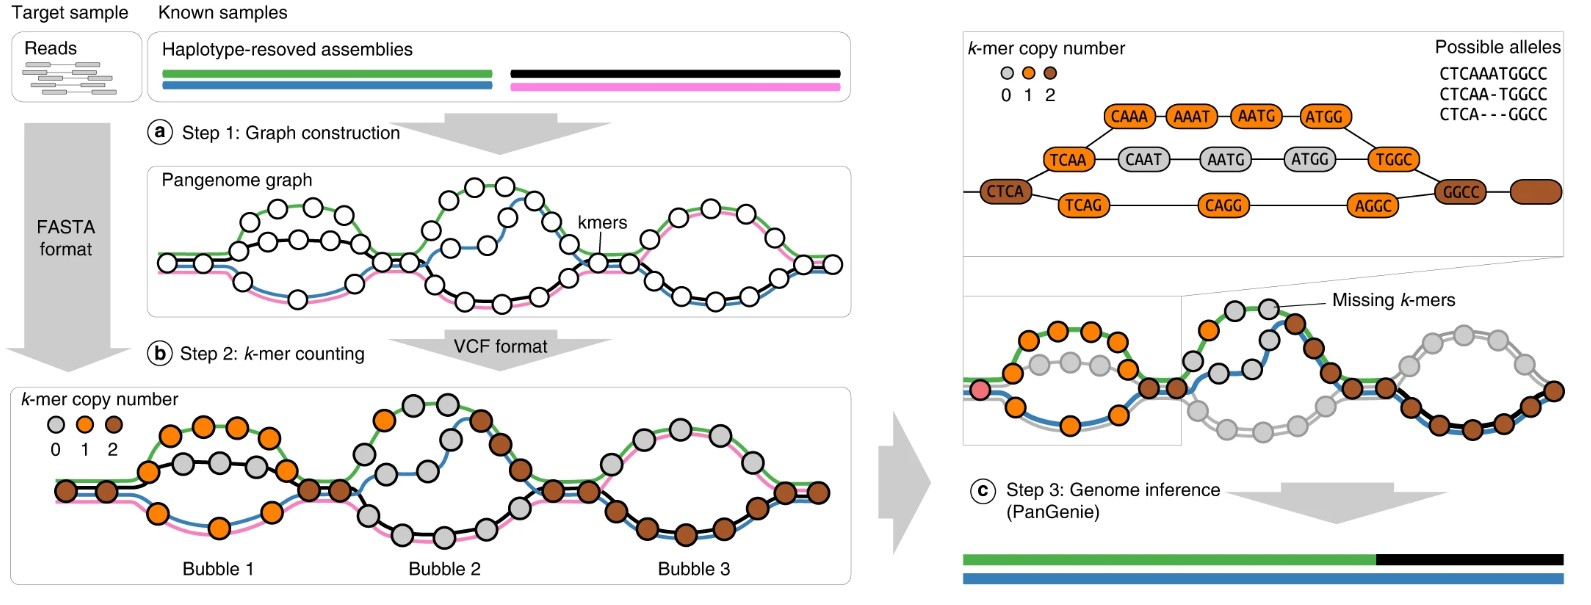
\includegraphics[scale=0.48]{figures/workflow of PanGenie.jpg}
	\caption{Workflow of PanGenie (Figure is taken from~\cite{elber2022PanGenie}, without changes, and is under a Creative Commons License.(\url{https://creativecommons.org/licenses/by/4.0/}))}
	\label{fig:PanGenie} % \ref{this label}
\end{figure}
\clearpage

\section{Spaced seeds}
Spaced seeds are an enhancement over traditional contiguous seeds used in computational biology, particularly in the context of sequence alignment and matching algorithms~\cite{BestHitsOf11101}. They are crucial for improving the sensitivity and efficiency of these processes.
\subsection{Definition}
Spaced seed is composed of 0s and 1s, where 0 represents a ``don't care'' position, and 1 represents a ``care'' position. For example, a spaced seed can be represented as 1001110, where 1s indicate positions that require a match, and 0s represent ``don't care'' positions. The weight of a spaced seed, denoted as $W$, is the number of 1s in the seed. The length, or span, is the total number of 0s and 1s combined. 

\subsubsection{Traditional contiguous seeds}
In sequence alignment, a contiguous seed is a continuous string of characters (nucleotides or amino acids) used as a basic unit or pattern for scanning and matching sequences. For example, a seed might be a simple string like ``ATCTCGA'' or ``AACTCG''.

\subsubsection{Spaced seeds}
Unlike contiguous seeds, spaced seeds include specific positions that are designated as ``don't care'' or gaps, interspersed between required matches.For instance, ``1100111''.
\vspace{3em}

In the notation introduced~\cite{SensSpacedSeed}, a spaced seed can be represented by its shape, denoted as $Q$. The weight $W$ of the seed is denoted by $\left | Q \right |$, and the length or span $s(Q)$ = max($Q$)+1. For instance, a seed $Q=110011$, then $Q=\{0, 1, 4, 5\}$ if we count from index 0, span $s(Q)=6$ and weight $\left | Q \right | = 4$ . For any integer $i$ and shape $Q$, the positioned shape $i+Q$ is the set $\{i+j:j\in Q\}$.
\vspace{2em}

\textbf{Example 2.1.} Let $Q=\{0, 1, 4, 5\}$ be a shape of the seed. Then, the seed is 110011. It's weight is $\left | Q \right | = 4$ and $s(Q)=7$ be the span. We assume the string $S=$ ATCAACGTA.
\vspace{2em}

\begin{center}   
\begin{tabular}{ccccccccccc}
 & & 0 & 1 & 2 & 3 & 4 & 5 & 6 & 7 & 8\\
 \midrule
S& & A & T & C & A & A & C & G & T & A\\
Q& & 1 & 1 & 0 & 0 & 1 & 1 \\
S[0+Q] & & A & T & & & A & C & &\\
S[1+Q] & & & T & C & & & C & G & &\\
\end{tabular}
\end{center}
\vspace{2em}

In \textbf{Example 2.1}, we can get that S[2+Q] = CAGT. By shifting the seed position with $i$, we can get the corresponding resulting strings, where $0\leq i\leq 3$

\subsection{Seed optimization}
To select the best seed, there are many adjustable parameters, such as weight and length. To evaluate the quality of each seed, we need to find a good metric for assessment~\cite{ChoiGoodSeed}. For instance, given $l=61$ and $w=41$, there are $\binom{61}{41} \approx 6 * 10^{15}$ different seed combinations. If we want to calculate the quality of all seeds, it will take a considerable amount of time. In the following sections, we'll describe metrics can be used to evaluate a good spaced seeds and introduce an algorithm for selecting good seeds.

\subsubsection{Sensitivity of spaced seeds}
Sensitivity in the context of bioinformatics and sequence alignment is crucial as it defines the ability of a seed or algorithm to correctly identify and match similar segments between biological sequences. This is particularly important when distinguishing between sequences that share common ancestry or functional similarities. Enhanced sensitivity allows researchers to detect subtle genetic variations that might have significant biological implications.

Let $S=s_1s_2\ldots$ be an infinite Bernoulli random sequence in which $S[i]:=s_i$ takes only two values, 1 or 0 with probability $p$ and $q:=1-p$ respectively~\cite{SensSpacedSeed}. The seed $Q$ is considered to hit $S$ at position n if
\begin{equation}
S[n-L+i_1+1]=S[n-L+i_2+1]= \ldots =S[n-L+i_w+1]=1,
\end{equation}
$n-L+i_w+1=n$. Here, we define the ending position as the hitting position. Let $Q_n:=Q_n(p)$ represent the probability that $Q$ hits $S$ before or at position $n$. Then, we seek an optimal seed with a given weight $w$ that maximizes the hitting probability $Q_n$ for given $n$ and $p$.

An algorithm has been proposed to accelerate the computation time of seed sensitivity. Using dynamic programming and recurrence relation, some of the equations can be proven to reduce computation time from exponential to polynomial~\cite{sensDP}.

In the above content, the computation of sensitivity has been improved. However, the overall time complexity remains exponential. A new metric presented by Ilie and Ilie~\cite{SpEED} is called overlap complexity, which experimental results have shown to be highly correlated with sensitivity. Moreover, the calculation of overlap complexity can be performed in polynomial time.

\subsubsection{Overlap complexity of spaced seeds}
The hits of a seed can overlap, but overlapping hits will detect only a single local alignment. Thus, the sensitivity of a seed is inversely proportional to the number of overlapping hits, given that the expected number of hits is the same for all seeds. Consequently, good seeds should have a low number of overlapping hits.

The equation of overlap complexity is formally defined as follows:
\begin{equation}
    OC(s) = \sum\limits_{i = 1}^{l-1}2^{\sigma[i]}
\end{equation}
where $\sigma[i]$ represents the number of pairs of ones that are aligned together when seed s is shifted by $i$ positions. In other words, this indicates the number of pairs of 1's separated by a distance of $i$ in s. Many tools for generating optimal spaced seeds implement the overlap complexity as metric.

\section{Related tools}
\subsection{SpEED}
Ilie and Ilie's algorithm is a well-known approach in genotyping that requires a fixed seed length as an input parameter. However, determining the optimal seed length remains a challenge. To address this, Ilie et al. proposed a heuristic algorithm that derives a suitable seed length within a specified range (min and max) by executing the algorithm multiple times with random seed lengths. This method has been implemented in the software SpEED, which can compute highly sensitive multiple spaced seeds in a few seconds.

SpEED's implementation demonstrates its capability by efficiently finding multiple spaced seeds up to a weight of 18. This rapid computation makes it a valuable tool in genotyping applications where sensitivity is critical. Despite its effectiveness, the challenge arises when dealing with mid-size k-mers, such as those used in PanGenie, which typically have a weight of 31. It remains uncertain whether SpEED can identify an optimal single seed for this weight, given the complexity of the problem.

\subsection{Rasbhari}
Lars Hahn et al. demonstrate that the overlap complexity of a pattern set, as introduced by Ilie and Ilie, is closely linked to the variance in the number of matches between two related sequences based on this pattern set. They suggest an improved hill-climbing algorithm designed to optimize pattern sets for tasks such as database searching, read mapping, and alignment-free sequence comparison of nucleic acid sequences. They named their implementation of this algorithm rasbhari. Depending on the application, rasbhari can be used to either minimize the overlap complexity of pattern sets, enhance their sensitivity for database searching, or reduce the variance in the number of pattern-based matches in alignment-free sequence comparisons.

\subsection{Jellyfish}
 ``k-mer'' refers to all possible substrings of length k that are contained within a sequence. Counting k-mers involves tallying how many times each possible k-mer appears in a given sequence. The process starts by sliding a window of length k along the sequence one base at a time, extracting every possible k-mer until the end of the sequence is reached. For instance, from the sequence ``ATCGA'', the 3-mers extracted would be ``ATC'', ``TCG'', and ``CGA''.

The conventional method utilizes a dictionary, with k-mers as keys and their respective counts as values. Yet, the emergence of high-throughput sequencing technologies, like next-generation sequencing (NGS), which generate an enormous amount of short sequences, necessitates the optimization of both time and memory consumption.

To tackle this challenge, the primary strategies for k-mer counting involve the use of hash tables, sorting algorithms, bloom filter. Moreover, Jellyfish utilizes parallel computing, allowing multiple threads to process parts of the sequence data simultaneously, significantly speeding up the k-mer counting process. Instead of a standard hash table, Jellyfish uses an enhanced data structure that minimizes memory usage while maintaining fast access times. This structure supports concurrent access by multiple threads without extensive locking, making it highly efficient for multi-core processors.

\chapter{Research Methodology}
\section{Spaced seeds generation}
In previous research, Yi-Tsung developed PalindromeSpEED, a modified version of SpEED, to generate palindrome spaced seeds. Although it showed improvements in genotyping results, there is still room for further enhancement in the quality of spaced seeds.

\subsection{Canonical form}
The canonical form of k-mers is a fundamental concept in bioinformatics, especially in DNA sequence analysis, which standardizes the handling and comparison of k-mers across different datasets and computational processes. This standardization is crucial for reducing complexity and enhancing the efficiency of genetic analyses such as k-mer counting, sequence alignment, and genome assembly.

For any given k-mer, the canonical representation is defined as the smaller (or lexicographically earlier) value between the k-mer and its reverse complement. Since DNA is double-stranded with each strand being complementary to the other, a sequence and its reverse complement (the sequence read in the opposite direction with complementary bases—adenine (A) pairing with thymine (T), and cytosine (C) pairing with guanine (G)) convey the same genetic information. Thus, this representation helps standardize k-mers by considering both the sequence and its reverse complement, ensuring consistent analysis.
\vspace{2em}

\textbf{Example 3.1.} Let a k-mer be ``AGCTA''. Its reverse complement is ``CTAGCT''. In the canonical representation, we compare ``AGCTAG'' and ``CTAGCT'' lexicographically and choose the one that comes first, which in this case is ``AGCTAG''.
\vspace{1em}

When counting k-mers or searching for k-mers within genomic data, using the canonical form ensures that each k-mer is represented uniquely, regardless of the direction in which it is read.

\subsection{Palindrome spaced seeds}
According to the previous section, we used the canonical form of k-mers, ensuring that our reverse strand is equivalent. However, when we use spaced seeds to generate k-mers, the reverse strand may not necessarily be equivalent.
\vspace{2em}

\textbf{Example 3.2.} Consider the spaced seed is 111001, and the DNA sequence ATTACG on the forward strand, then CGTAAT on the reverse strand. As the result, the resulting 4-mer is ATTG on the forward strand, and the reverse strand is CGTT. Their canonical forms are ATTG and AACG, which are not equivalent.
\vspace{1em}

\textbf{Example 3.3.} We consider using a palindrome spaced seed 110011, and the DNA sequence is the same with \textbf{Example 3.2}. The resulting 4-mer is ATCG on the forward strand, and the reverse strand is CGAT. Their canonical forms are ATCG and ATCG, which are equivalent.
\vspace{1em}

In the above example, we can see that using a palindrome spaced seed guarantees that the canonical forms of the forward strand and reverse strand are equal.

Palindrome spaced seeds are defined as follows. For a spaced seed $S=s_0,s_1,s_2,...,s_{n-1}$, where $s_i$ be the elements of the seeds and the length is $n$. A palindrome spaced seed is $\forall i \in [0, \lfloor \frac{n}{2} \rfloor]$, $s_i = s_{n-i-1}$, which implies that the elements of the seed are symmetrical around the center. Additionally, it is important to note that this study will exclude spaced seeds with leading and trailing zeros. This is because leading and trailing zeros in spaced seeds do not affect the composition of the selected k-mers.  

The original author of MaskedPanGenie used palindrome spaced seed as the mask. However, the author generated half of the seed using SpEED and manually created the other half to follow the rule of palindrome. This approach presents a problem because, while the seeds generated by SpEED have high sensitivity, manually converting them into a palindrome format significantly reduces their sensitivity.

\subsection{PalindromeRasbhari}
Currently, there are many tools available for generating spaced seeds, but few focus on palindrome spaced seeds. Among these, Cheng has developed a tool that generates palindrome seeds based on the SpEED algorithm~\cite{garyMaskedPanGenie}. In this study, we have also developed our own tool, PalindromeRasbhari, which is based on another spaced seed generation tool, Rasbhari.

The program allows users to define the seed length and weight. It begins with a predefined pattern or a random seed pattern and then proceeds with iterative optimization. Through these iterations, we can obtain an optimized seed. Furthermore, PalindromeRasbhari can generate not just a single seed, but also multiple spaced seeds for use in similarity and sequence alignment analysis. It can create a custom-sized pattern set and maximize the average sensitivity of that pattern set.

In the SpEED algorithm, it randomly swaps two positions, i and j, of the seed. At the swap positions, if the original value is 0, it is converted to 1; if the original value is 1, it is converted to 0. Using overlap complexity (OC) as a metric, if the OC after swapping is smaller than the original OC, we take the swapped seed as the new seed and perform the swap operation again. This process continues until the seed reaches the desired sensitivity.
Howerver, SpEED uses the original hill-climbing algorithm, which calculate OC for all pattern sets. Rasbhari, on the other hand, uses a modified hill-climbing algorithm. Instead of examining all possible seed patterns, it prioritizes those patterns that contribute the most to the OC.

PalindromeRasbhari requires parameters, specifically the number of don't care position (-d), seed weight (-w), similarity level (-p), iteration of optimization for seed (-t). To compare the results with previous methods (Häntze and Cheng), we used PalindromeRasbhari to generate seeds with the same length and weight. The first case is a length of 41 and a weight of 31, and the second case is a length of 39 and a weight of 25. We can observed that palindrome spaced seeds we generated by PalindromeRasbhari have higher sensitivity(see Table\ref{table:PalindromeRasbhari}).
\vspace{2em}
\begin{table}[h!]
	\centering
	\begin{tabular*}{\textwidth}{@{\extracolsep{\fill}}ccc@{\extracolsep{\fill}}}
        \toprule
        Method & Palindrome Spaced Seed & Sensitivity\\
        \midrule
        Original~\cite{haimo2023MaskedPanGenie}&11101110110110101111111110101101101110111&0.826843\\
        Original~\cite{haimo2023MaskedPanGenie}&11111010110110111011111011101101101011111&0.838849\\
        PalindromeSpEED~\cite{garyMaskedPanGenie}&11111110110101110011111001110101101111111&0.856148\\
        \textbf{PalindromeRasbhari} &11110111011011110101110101111011011101111&\textbf{0.859432}\\
        \midrule 
        Original~\cite{haimo2023MaskedPanGenie}&111010011010011101111101110010110010111&0.94561\\
        Original~\cite{haimo2023MaskedPanGenie}&111011100101100101111101001101001110111&0.955228\\
        PalindromeSpEED~\cite{garyMaskedPanGenie}&111110110110001101010101100011011011111&0.958913\\
        \textbf{PalindromeRasbhari} &111110101101001100111001100101101011111&\textbf{0.959918}\\
        \bottomrule 
	\end{tabular*}
	\caption{Seed generated by original method, PalidromeSpEED and PalindromeRasbhari.}
	\label{table:PalindromeRasbhari}
\end{table}

\section{Fast spaced seed hashing}
Hashing plays an important role in k-mer counting, and hash table structures, a type of hash-based data structure, provide an effective method for carrying out these operations. For contiguous k-mers, this process is relatively straightforward because the hash value can be computed by extending the hash value calculated at the previous position, as they share  $k-1$  symbols. Consequently, indexing all contiguous k-mers in a string can be a highly efficient process. However, these observations do not apply when using spaced seeds. As a result, enhancing the performance of spaced seed hashing algorithms would improve the speed of computation. 

Because the computation time for k-mer counting in MaskedPanGenie is still relatively high, I have referred to the FSH algorithm to improve the original hashing function~\cite{FSH}.

In this method, we use the Rabin-Karp rolling hash. First, we need to define the encoding function. Let $encode(A)=00$, $encode(C)=01$, $encode(G)=10$, $encode(T)=11$. Based on the encoding function, we can determine the encodings of the symbols of the Q-gram. 

\textbf{Example 3.4.}
\begin{center}   
\begin{tabular}{ccccccc}
S[0+Q] & A & T & A & C & G & T\\
$encodings$ & 00 & 11 & 00 & 01 & 10 & 11\\
\end{tabular}
\end{center}
\vspace{1em}

The hashing function defined as $h(S[0+Q]) = encode(A)*4^0+encode(T)*4^1+encode(A)*4^2+encode(C)*4^3+encode(G)*4^4+encode(T)*4^5$. The reason for using powers of 4 here is that DNA sequences are composed of four symbols: A, C, G, and T. Powers of 2 can be implemented using bit shifts. In \textbf{Example 3.4}, we can obtain the hash result for ATACGT, represented in Little-endian as 111001001100.

When we apply the spaced seed mask to the sequence, we may find that some positions have already been calculated in a previous hash. We can utilize these precomputed positions to increase the speed of hashing. We define  $C_j$  as the value when processing position i of sequence S, where we aim to reuse the hash value already computed at position  $i-j$.  

\section{MaskedPanGenie}
Under Häntze's improvements, MaskedPanGenie can use spaced seeds, but the execution time becomes significantly slower when supporting spaced seeds. Cheng's improvements integrated the k-mer counting calculations into the MaskedPanGenie code, addressing the original version's approach where k-mer counting was first executed by Jellyfish, outputted to a fasta file, and then inputted into MaskedPanGenie. Due to the large size of DNA sequence files, this method required multiple file reads, significantly increasing I/O time. By addressing this issue, the overall execution time was reduced. However, we observed that there are still areas for improvement in k-mer counting. During the hashing process of spaced seeds, although there are fewer overlapping positions compared to contiguous seeds, there are still many redundant overlaps with spaced seeds. These redundancies increase the computation time.

To understand the modifications made, we need to analyze MaksedPanGenie's source code, which is broadly divided into four sections.
\vspace{1em}

1. Build a pangenome graph using a given VCF file.
\vspace{1em}

2. Determine the k-mer counts in the reads and the pangenome graph.
\vspace{1em}

3. Determine unique k-mers.
\vspace{1em}

4. Build HMM and calculate the most likely genotypes.
\vspace{1em}

In step 1, build the pangenome graph, noting that the bubbles in the graph depend on the spaced seed length. In step 2, count k-mers in the reads and pangenome. This step is the main modification of this research. In step 3, MaskedPanGenie initially counts all k-mers within each bubble and then compares these counts to those across the entire pangenome. If a k-mer's count is the same in both, it uniquely belongs to the tested variant bubble. In the final step, create and run an HMM.

In the original method of step 2, the author includes the MaskedJellyfish library, which uses the same hash function as that used with contiguous k-mers. As a result, it involves a lot of redundant computation. We utilize the method introduced in Chapter 3.2 to reduce the number of symbol copies and improve overall performance. First, the symbols ``A'', ``C'', ``G'' and ``T'' are encoded as ``00'', ``01'', ``10'' and ``11'', respectively. Second, we identify the optimal positions of previously known k-mers while traversing the sequence, which is $C_j$ as discussed in the previous section. Third, after computing the previous hashes, we can use  $C_j$  to accelerate the hash calculations. 

\chapter{Data}
\section{Pangenome reference}
We utilized sequencing data from the GIAB consortium~\cite{GIAB}, 1000 Genomes Project~\cite{1000Genomes}, and data from the Human Genome Structural Variation Consortium~\cite{HGSVC}. The haplotype-resolved pangenome graph was constructed for the same group of 11 unrelated individuals, including NA19238, NA19239, HG00731, HG00732, HG00512, HG00513, NA12878, HG02818, HG03125, NA24385, HG03486, as reported by Hartmut Häntze. The author combined variation calls and filtered for variants present in at least one of the 11 samples, ensuring that the alternative genotype was known for at least 80\% of the samples. The number of variants covered by the pangenome graph was reported according to Hartmut Häntze's findings.

For the leave-one-out cross-validation, subsets of the pangenome were used, excluding the haplotypes of the individual being tested. These excluded haplotypes served as the ground truth. Variants not covered by either the true haplotype of the tested individual or the remaining haplotypes in the pangenome were excluded from the analysis.

\section{Reads}
The test data comprised reads from nine individuals selected from the eleven used to construct the pangenome reference. All reads were sequenced as part of the same BioProject using an Illumina HiSeq X Ten system, employing a whole-genome sequencing strategy with 30x coverage and a paired-end layout. The two remaining individuals were not included in the BioProject and were excluded from this study to avoid potential noise from different sequencing platforms. 

For the leave-one-out cross-validation, subsets of the pangenome were utilized, excluding the haplotypes of the individual being tested. These excluded haplotypes were treated as the ground truth. Any variants not present in the true haplotype of the tested individual or the remaining haplotypes in the pangenome were omitted from the analysis.

\vspace{2em}

\begin{itemize}
    \item HG00731: SRR7782675(Puerto Rico - American Ancestry, Male)
    \item HG00732: SRR7782676(Puerto Rico - American Ancestry, Female)
    \item HG00512: SRR7782672(Han Chinese - East Asian Ancestry, Male)
    \item HG00513: SRR7782673(Han Chinese - East Asian Ancestry, Female)
    \item NA19238: SRR7782690(Nigeria - African Ancestry, Female)
    \item NA19239: SRR7782691(Nigeria - African Ancestry, Male)
    \item NA12878: SRR7782683(Utah - European Ancestry, Female)
    \item HG02818: SRR7782682(The Gambia - African Ancestry, Female)
    \item NA24385: SRR7782670(Ashkenazim Jewish Ethnicity, Male)
\end{itemize}
\vspace{2em}


To evaluate the impact of spaced seeds on reads with lower coverage, the author downsampled the reads to a target coverage of 5x. The reads were subsequently aligned to the reference genome using BWA-MEM~\cite{BWAMEM} and processed with Picard's DownsampleSam, which reduced the coverage by one-sixth. This tool also handled unaligned reads by randomly downsampling them to the same fraction.
\chapter{Results}
\section{Spaced seed on Genotyping}
\subsection{Sensitivity}
Different spaced seeds can affect genotyping results. We conducted experiments on reads from nine samples with coverages of 5-fold and 30-fold. First, we compared the sensitivity of spaced seeds generated by PalindromeSpEED and PalindromeRasbhari. We divided the experiment into three parts: length 41, weight 31; length 51, weight 31; and length 61, weight 31. Seed1, seed3 and seed5 are generated by PalindromeSpEED, and seed2, seed4 and seed6 are generated by PalindromeRasbhari. Also, a contiguous seed pattern seed0. It is worth mentioning that the sensitivity of seed5 and seed6 cannot be calculated due to the need for additional time and memory resources. Given these limitations, seed5 and seed6 are generated using the spaced seed from the PalindromeRasbhari tool with the best overlap complexity. See Table \ref{table:Length variation}

\begin{table}[ht]
    \centering
    \begin{tabular}{|c|c|c|}
    \hline
      Seeds&Seeds Pattern&Sensitivity\\
    \hline
        seed0&1111111111111111111111111111111&0.624134\\
    \hline
        seed1&11111110110101110011111001110101101111111&0.856148\\
    \hline
        seed2&11110111011011110101110101111011011101111&0.859432\\
    \hline      
        seed3&111111101010011100010110010011010001110010101111111&0.860626\\
    \hline
        seed4&111111001101010100101100111001101001010101100111111&0.863834\\
    \hline
        seed5&1111000110010100101000100110111110110010001010010100110001111&X\\
    \hline

        seed6&1111100110001010100101100100011100010011010010101000110011111&X\\
    \hline
    \end{tabular}
    \caption{Spaced seeds and sensitivity}
    \label{table:Length variation}
\end{table}

\subsection{Genotyping results}
In this section, we compare the impact of seed1 through seed6 on genotyping results, using three different seed lengths. For each seed length, we have two seed patterns. By using seeds with the same length, we observe how sensitivity affects the outcomes. The results are based on experiments conducted on 9 samples, representing the average values of these 9 samples and standard error of the mean. Table \ref{table:5x-results} and Table \ref{table:30x-results} present the genotyping results at 5-fold and 30-fold coverage. According to the results, it can be observed that seed0, a contiguous seed, performs the worst, highlighting the superior effectiveness of spaced seeds. Additionally, we can see that seed3 and seed4 performs better, confirming previous findings that a seed with length 51 and weight 31 yields the best genotyping results. Furthermore, seed4, generated using PalindromeRasbhari, produced the best outcomes. 

\section{Performance of MaskedPanGenie}
\subsection{Runtime}
We compared the runtime of our proposed method with Cheng's improved version of MaskedPanGenie(Fast-MaskedPanGenie)~\cite{garyMaskedPanGenie}. Tests were conducted on a Linux server equipped with a single AMD Ryzen™ 9 5950X processor, which has 16 hyper-threaded physical cores running at a clock rate of 3.4GHz, and 128GB of RAM. 

The spaced seed setting remains the same as those used in Cheng's experiment, which is 111111101010011100010110010011010001110010101111111 (length = 51, weight = 31). The data used for assessment was NA12878 with 30-fold coverage. Within the MaskedPanGenie framework, the genotyping step can be divided into four sections
\begin{enumerate}[label=(\alph*)]
\item Read the input files.
\item Determine the k-mer counts in the reads and the pangenome graph.
\item Determine unique k-mers.
\item Build HMM and calculate the most likely genotypes.
\end{enumerate}

From Table \ref{table:RuntimeFSH}, it can be observed that the total execution time has decreased. The improvement lies in our enhancement of the hashing method during the k-mer counting step, reducing redundant steps by calculating the specific positions of the spaced seed symbols. The execution times for steps (a), (c), and (d) are the same as Fast-MaskedPanGenie because these steps do not include k-mer counting. Step (b), which involves k-mer counting, shows that our method has reduced the time by more than 20\%.

However, the FSH algorithm includes a preprocessing stage to identify the optimal positions of known k-mers during sequence traversal. This step aims to minimize the number of symbols that must be processed. The additional computational effort from this preprocessing stage affects the overall runtime.
\begin{table}[ht!]
	\centering
	\begin{tabular*}{\textwidth}{@{\extracolsep{\fill}}cccccc@{\extracolsep{\fill}}}
        \toprule
         & Reading & Counting & Unique & HMM & Total\\
         Method & Input & & & &\\
        \midrule
        Fast-MaskedPanGenie& 11min & 64min & 4min & 94min & 2h:53min\\
        FSH-MaskedPanGenie& 11min & 48min & 4min & 94min & 2h:37min\\
        \bottomrule 
	\end{tabular*}
    \caption{Runtime for genotyping NA12878 with 30-fold coverage.}
	\label{table:RuntimeFSH}
\end{table}

\subsection{Memory}
In the memory comparison, the test data used are the same as those in Fast-MaskedPanGenie. These datasets are HG00512, HG00731, NA12878, and NA19238, each with 30-fold coverage, totaling four datasets. Additionally, memory usage was analyzed under identical conditions to ensure a fair comparison of performance between the two methods.

The memory usage of MaskedPanGenie employing the FSH algorithm is higher compared to the original Fast-MaskedPanGenie (Table \ref{table:Memory-FSH}). This increase is due to the FSH method utilizing dynamic programming to compute hash values and needing to record the optimal positions of spaced seeds. Consequently, this process generates additional memory overhead. This increase in memory consumption is a trade-off for the improved runtime performance and memory usage in k-mer counting, as it allows for more efficient handling of spaced seeds despite the additional computational complexity.
Notably, the increase in memory usage compared to Fast-MaskedPanGenie is not significant.

\begin{table}[ht!]
	\centering
	\begin{tabular*}{\textwidth}{@{\extracolsep{\fill}}ccccc@{\extracolsep{\fill}}}
        \toprule
         & HG00512 & HG00731 & NA12878 & NA19238 \\
         Method & & & & \\
        \midrule
        Fast-MaskedPanGenie& 80.0799GB & 80.2827GB & 80.2818GB & 79.6233GB\\
        FSH-MaskedPanGenie& 82.5429GB & 82.7016GB & 82.7093GB & 82.0462GB\\
        \bottomrule 
	\end{tabular*}
	\caption{Memory usage for Fast-MaskedPanGenie and FSH-MaskedPanGenie across four samples.}
	\label{table:Memory-FSH}
\end{table}

\begin{table*}[ht!]
\begin{tabular*}{\textwidth}{@{\extracolsep{\fill}}llllll@{\extracolsep{\fill}}}
\toprule
   &         &               wGC &         Precision &            Recall &           F-score \\
Variant & Seed &                   &                   &                   &                   \\
\midrule
indel & seed0  & 0.774(SE=0.009) & 0.817(SE=0.007) & 0.722(SE=0.012) & 0.767(SE=0.009) \\
   & seed1 & 0.817(SE=0.008)&  0.803(SE=0.007)&  0.761(SE=0.012)&  0.781(SE=0.009)\\
   & seed2 & 0.817(SE=0.008) & 0.804(SE=0.007) &0.759(SE=0.011) & 0.781(SE=0.009)\\
   & seed3 & 0.823(SE=0.008)& 0.790(SE=0.008)& 0.763(SE=0.012)& 0.776(SE=0.010)\\
   & seed4 & 0.825(SE=0.008) & 0.792(SE=0.008) & 0.763(SE=0.012)&  0.777(SE=0.010)\\
   & seed5 & 0.816(SE=0.009)&  0.774(SE=0.012)&  0.753(SE=0.013)&  0.763(SE=0.011)\\
   & seed6 & 0.815(SE=0.012)&  0.772(SE=0.013)&  0.755(SE=0.015)&  0.763(SE=0.013)\\
\midrule
snv & seed0  & 0.877(SE=0.014)  & 0.896(SE=0.015)  & 0.842(SE=0.018)  & 0.868(SE=0.016) \\
   & seed1 &0.896(SE=0.010)&  0.896(SE=0.012)&  0.861(SE=0.013)&  0.878(SE=0.012)\\
   & seed2 &0.896(SE=0.012)&0.898(SE=0.014)& 0.860(SE=0.016)& 0.879(SE=0.014)\\
   & seed3 & 0.904(SE=0.010)& 0.894(SE=0.013)& 0.869(SE=0.013)& 0.881(SE=0.012)\\
   & seed4 & 0.905(SE=0.011)&  0.895(SE=0.013)&  0.871(SE=0.014)&  0.883(SE=0.013)\\
   & seed5 & 0.901(SE=0.013)&  0.883(SE=0.016)&  0.864(SE=0.016)&  0.873(SE=0.016)\\
   & seed6 &  0.901(SE=0.013)&  0.886(SE=0.017)&  0.868(SE=0.016)&  0.877(SE=0.017) \\
\midrule
sv & seed0  & 0.650(SE=0.010) & 0.613(SE=0.008)  & 0.579(SE=0.011)  & 0.596(SE=0.009) \\
   & seed1 & 0.669(SE=0.009)&  0.610(SE=0.008)&  0.592(SE=0.009)&  0.601(SE=0.008)\\
   & seed2 & 0.670(SE=0.008) & 0.609(SE=0.010) & 0.592(SE=0.010) & 0.600(SE=0.009)\\
   & seed3 & 0.676(SE=0.009)&0.603(SE=0.010)&0.596(SE=0.010)&0.600(SE=0.009)\\
   & seed4 & 0.676(SE=0.008) & 0.604(SE=0.009)&  0.596(SE=0.010)&  0.600(SE=0.009)\\
   & seed5 & 0.676(SE=0.011)&  0.595(SE=0.014)&  0.594(SE=0.013)&  0.594(SE=0.013)\\
   & seed6 & 0.675(SE=0.013)&  0.597(SE=0.019)&  0.595(SE=0.016)&  0.596(SE=0.017)\\
\bottomrule
\end{tabular*}
\caption{Genotyping results for seed1 through seed6 at 5-fold coverage 
\label{table:5x-results}}
\end{table*}

\begin{table*}[ht!]
\begin{tabular*}{\textwidth}{@{\extracolsep{\fill}}llllll@{\extracolsep{\fill}}}
\toprule
   &         &               wGC &         Precision &            Recall &           F-score \\
Variant & Seed &                   &                   &                   &                   \\
\midrule
indel & seed0  & 0.825(SE=0.015) & 0.889(SE=0.012) & 0.790(SE=0.022) & 0.836(SE=0.017) \\
   & seed1 & 0.876(SE=0.018)&  0.889(SE=0.012)&  0.790(SE=0.022)&  0.836(SE=0.017)\\
   & seed2 & 0.877(SE=0.018) & 0.890(SE=0.009) &0.790(SE=0.024) & 0.837(SE=0.017)\\
   & seed3 & 0.888(SE=0.019)& 0.881(SE=0.013)& 0.846(SE=0.030)& 0.863(SE=0.022)\\
   & seed4 & 0.890(SE=0.018) & 0.883(SE=0.028) & 0.847(SE=0.032)&  0.865(SE=0.022)\\
   & seed5 & 0.890(SE=0.019)&  0.878(SE=0.013)&  0.846(SE=0.032)&  0.862(SE=0.022)\\
   & seed6 & 0.890(SE=0.012)&  0.880(SE=0.013)&  0.847(SE=0.030)&  0.863(SE=0.017)\\
\midrule
snv & seed0  & 0.877(SE=0.014)  & 0.896(SE=0.015)  & 0.842(SE=0.018)  & 0.868(SE=0.016) \\
   & seed1 &0.962(SE=0.002)&  0.977(SE=0.003)&  0.956(SE=0.004)&  0.966(SE=0.003)\\
   & seed2 &0.964(SE=0.020)&0.978(SE=0.004)& 0.956(SE=0.004)& 0.967(SE=0.004)\\
   & seed3 & 0.970(SE=0.003)& 0.976(SE=0.003)& 0.963(SE=0.005)& 0.969(SE=0.004)\\
   & seed4 & 0.973(SE=0.002)&  0.978(SE=0.003)&  0.965(SE=0.004)&  0.971(SE=0.003)\\
   & seed5 & 0.972(SE=0.004)&  0.973(SE=0.003)&  0.965(SE=0.006)&  0.969(SE=0.004)\\
   & seed6 &  0.972(SE=0.003)&  0.974(SE=0.003)&  0.964(SE=0.005)&  0.969(SE=0.004) \\
\midrule
sv & seed0  & 0.650(SE=0.010) & 0.613(SE=0.008)  & 0.579(SE=0.011)  & 0.596(SE=0.009) \\
   & seed1 & 0.705(SE=0.015)&  0.664(SE=0.012)&  0.633(SE=0.018)&  0.648(SE=0.013)\\
   & seed2 & 0.706(SE=0.015) & 0.665(SE=0.010) & 0.633(SE=0.010) & 0.649(SE=0.009)\\
   & seed3 & 0.717(SE=0.015)&0.664(SE=0.011)&0.642(SE=0.020)&0.653(SE=0.014)\\
   & seed4 & 0.719(SE=0.015) & 0.666(SE=0.009)&  0.643(SE=0.016)&  0.654(SE=0.009)\\
   & seed5 & 0.724(SE=0.016)&  0.664(SE=0.011)&  0.648(SE=0.021)&  0.656(SE=0.015)\\
   & seed6 & 0.724(SE=0.013)&  0.665(SE=0.011)&  0.648(SE=0.016)&  0.656(SE=0.014)\\
\bottomrule
\end{tabular*}
\caption{Genotyping results for seed1 through seed6 at 30-fold coverage 
\label{table:30x-results}}
\end{table*}



\chapter{Discussion \& Future Work}
Our proposed method improves the overall execution time, especially when processing multiple samples, leading to even greater reductions in total runtime. The primary improvement is focused on the k-mer counting for spaced seeds. As shown in Table \ref{table:RuntimeFSH}, the execution time for the HMM remains unchanged and is the most time-consuming part of the genotyping process. To achieve a substantial reduction in computation time, it is crucial to optimize the HMM calculations as well. There are currently several different versions of HMM available, and utilizing GPUs might be a viable approach~\cite{FastHMM}. Research indicates that GPU-based HMM implementations can significantly outperform their CPU counterparts in terms of execution time, offering a potential solution for further optimization.

In terms of memory usage, an effective approach could be the DSK (Disk Streaming of k-mers) algorithm~\cite{DSK}, which is known for its low memory requirements. DSK only requires a fixed, user-defined amount of memory and disk space. This approach achieves a balance between memory, time, and disk usage by partitioning the multi-set of all k-mers present in the reads and saving these partitions to disk. Each partition is then loaded into memory separately in a temporary hash table, where k-mer counts are processed.

Another potential improvement could be in the seed pattern. While Häntze's and Cheng's improved versions of MaskedPanGenie utilize spaced seeds, there are other seed patterns that can be applied, such as subset seeds~\cite{SubsetSeeds}. Based on the characteristics of DNA sequences, subset seeds can be used where AT is considered a match and CG is considered a match. By experimenting with different seed pattern combinations and considering sensitivity, the feasibility of subset seeds can be determined through further experimentation.

\chapter{Conclusion}
In this study, we present an improved version of MaskedPanGenie, which offers better accuracy and speed. We introduced a new method for k-mer counting in the original MaskedPanGenie to eliminate redundant computations. Additionally, users can easily utilize our software to perform genotyping tasks. 

We also proposed a new method for generating palindrome spaced seeds, which offers better sensitivity. We conducted experiments with these new seeds to analyze their impact on genotyping results. If new metrics are adopted to evaluate the genotyping results, it could provide a more comprehensive exploration of the entire experiment.


\newpage
\AddToContents{Bibliography}
\printbibliography


\end{document}
